\section{Validation}

\subsection{Validation Methodology}

Validation combines dynamic tests with source inspection. Most
mechanism tests use directed, freestanding RISC-V workloads in
syscall-emulation mode, comparing feature-disabled and feature-enabled
configurations where applicable. Python checkers examine program
outputs, committed instruction traces, simulator traces, and
statistics to verify expected prediction, bypass, dependency, and
recovery behavior. Since the checkers were developed alongside the
implementation, passing results establish consistency with the
design for the tested scenarios rather than an independent proof
of correctness.

\subsection{Standalone LVP Validation}

Standalone LVP was evaluated with a dedicated regression suite in
RISC-V syscall-emulation mode. The six test modes cover stable and changing
values, multiple consumers, dependent-load chains, memory faults,
confidence thresholds, PC-window restrictions, invalid configurations,
and predictor-table aliasing. The retained runs report 772 passing
checks with no failures per run.

\subsubsection{Test Configurations and Checks}

The test driver uses four configurations: A (LVP disabled), B
(prediction only), C (LVP with dependent-load speculation), and CL
(speculation with detailed tracing). Configuration B separates
predictor training and lookup from speculative use, while CL enables
inspection of individual producer-consumer interactions. The
committed instruction traces for A, B, and C match in the tested
workloads.

The checker compares program checksums and committed instruction
traces, verifies prediction admission against confidence thresholds
and PC-window restrictions, and confirms that speculative consumer
loads are issued only in configuration C. It also checks dynamic
producer-consumer associations, recovery after incorrect predictions
are used, and the squashing of affected younger instructions.
Fetch2 branch-predictor cleanup is verified against the recorded
recovery redirects.

\subsubsection{Functional and Lifecycle Tests}

The main execution mode uses five directed workloads to exercise
different aspects of LVP behavior: stable values and successful
prediction (Stable), changing values and misprediction recovery
(Phase), multiple consumers of a predicted producer (Fan-out),
memory faults involving speculative consumers (Fault), and chains
of dependent loads in which a consumer can subsequently act as a
producer (Chain).

All five workloads passed every check in the main execution mode, with
473 passing checks and no failures in total. Together, they exercise
stable predictions, changes in prediction behavior, multiple
consumers, fault handling, and chains of dependent loads.

\subsubsection{Predictor Policy and Configuration Tests}

Five additional test modes reported 299 passing checks with no
failures. They cover confidence thresholds (1, 2, and 3), PC-window
restrictions, rejection of invalid configurations, confidence-counter
updates, and predictor-table aliasing. The confidence test verifies
that a mismatch decrements a saturated counter from 3 to 2 rather
than resetting it, while the alias test confirms that PCs separated
by 2,048 bytes map to the same entry in the default 1,024-entry
untagged predictor table.

\subsubsection{Recovery and Trace Validation}

Detailed LVP traces recorded 255, 255, 32, and 26 recovery
redirects for the phase, fan-out, fault, and chain workloads,
respectively. The checker verifies that every used incorrect
prediction is followed by exactly one recovery redirect and that
no redirect occurs without an accepted speculative consumer.

It also checks the event ordering:
\[
    \text{accept}
    <
    \text{validation}
    \leq
    \text{redirect}
    <
    \text{consumer squash}.
\]
The Fetch2 cleanup-hook count is checked against the number of
redirects and the \texttt{lvp.mispredictSquashes} statistic.
Additionally, committed speculative loads must have used correct
predictions, and consumers affected by recovery must be discarded
rather than committed from the old instruction stream. The
\texttt{lvp.mispredictSquashes} statistic counts recovery redirects,
not individual instructions discarded.

\subsubsection{Test Results and Limitations}

The six-mode standalone LVP regression suite reported 772 passing
checks with no failures per run. The tests cover prediction behavior,
dependent-load chains, fan-out, memory faults, predictor
configuration, confidence updates, and table aliasing. Detailed
traces also provide evidence for speculative-use tracking and
misprediction recovery in the tested workloads.

Several cases remain untested, including drain during recovery,
idling-enabled execution, and statistics reset while speculative
instructions remain in flight. The suite also does not exercise
multithreaded execution or branch predictors other than TournamentBP.
The speculative operand path is restricted to eligible integer loads.
Floating-point and vector loads, as well as store interactions beyond
the tested cases, remain outside the validated scope.

\subsection{ASTRA and V-ASTRA Validation}
\label{subsec:astra-vastra-validation}

ASTRA and V-ASTRA were validated using directed RISC-V workloads
and instrumented traces. Component-level tests examine predictor
updates, value-cache operations, candidate classification, and
older-store conflict handling. Separate end-to-end tests verify
that accepted V-ASTRA loads complete without issuing normal memory
requests. These checks distinguish candidate generation from
successful bypass: a correct candidate does not necessarily
guarantee that a load bypasses memory or commits correctly.

\subsubsection{ASTRA Predictor Tests}
\label{subsubsec:astra-validation}

Two complementary suites validate ASTRA. The first compares
ASTRA disabled, ASTRA in shadow mode, and shadow mode with detailed
logging. Across ten loads in seven
functions, it records 640 committed loads and reports 78 passing
checks. The checker replays logged lookups and updates against a
reference model of the predictor, verifying PC indexing, stride calculations,
LAT and SS updates, retirement-order training, and instruction
lifecycle accounting.

The second, targeted suite reports 340 passing checks across seven modes. These exercise cold
prediction, PC and stride-table aliasing, destructive conflicts,
wrong-path and fault handling, invalid configurations, and
coexistence with LVP. The alias tests verify the expected 2,048-byte
PC alias in the default 1,024-entry configuration.

\subsubsection{Value-Cache Validation}
\label{subsubsec:vcache-validation}

The value-cache suite reports 157 passing checks and no failures, divided among operations
(32), squash (34), fault (31), and non-interference (60).

The operations mode executes a 52-step directed sequence and checks
allocation, replacement, updates, store hits and misses, byte-validity
tracking, tag conflicts, cross-line behavior, and invalidation for
atomic and load-reserved/store-conditional operations. The checker
replays the observed value-cache operations and statistics against a
reference model. The squash and fault modes check that discarded or
faulting operations do not update the cache. The non-interference mode
compares disabled and shadow executions, including cycle counts, and
checks that diagnostic hits do not return incorrect data. In the LVP
phase, the checker observed 16,382
byte-valid hits and reported no incorrect diagnostic data. These results cover the tested cache operations and execution paths.

\subsubsection{V-ASTRA Candidate Validation and Strict Verification}
\label{subsubsec:vastra-candidate-validation}

The V-ASTRA suite reported 276 passing checks
with no failures. It covers candidate classification, older-store
conflicts, instruction discard and fault handling, and
non-interference between feature-disabled and shadow executions.

Strict verification separately compares byte-valid V-ASTRA candidate
data against values obtained through the ordinary memory path. Across
the retained tests, 5,605 candidate instances were verified with no
mismatches. This verification was performed with load bypass disabled.
It establishes agreement between candidate data and memory results,
but does not demonstrate successful memory bypass. Actual bypass
behavior is validated separately.

\subsubsection{Older-Store Negative Control}
\label{subsubsec:vastra-negative-control}

A negative-control experiment evaluates the importance of the
older-store scan. With the scan enabled, 14 conflicting loads were
rejected, and strict verification found no incorrect candidates
among 15 verified instances. Disabling the scan allowed six
byte-valid candidates containing stale data, all associated with
older overlapping stores still in flight.

With strict verification enabled, the same execution terminated
with the expected simulator panic because the predicted base was
correct but the candidate bytes differed from the values returned
by memory. These results demonstrate that the older-store scan
prevents this specific class of stale candidates and that strict
verification detects the injected failure.

\subsubsection{Actual Load-Bypass Validation}
\label{subsubsec:vastra-bypass-validation}

Actual load bypass is tested by comparing bypass-disabled and
bypass-enabled executions.
The checker compares program outputs and committed instruction traces,
and examines memory-access traces and bypass statistics. Across 17 modes,
the suite reported 297 passing checks with no failures. The tests
cover candidate classification, store and atomic conflicts,
discarded and faulting loads, fallback cases, split and special
accesses, syscall handling, LVP coexistence, and ordering and
configuration restrictions.

The synonym mode reported 18 passing checks but could not construct
a genuine virtual-address synonym in syscall-emulation mode.
Consequently, it does not validate the implementation's behavior
under virtual synonyms.

In the classify mode, 22 bypassed loads produced synthetic responses
without issuing normal memory requests or receiving memory responses.
The checker confirmed that each request was deleted exactly once and
that all loads completed without reported violations. Data-cache read
accesses decreased by 22, matching the suppressed requests, while
the value cache did not observe the bypassed loads.

\subsubsection{Validation Limitations}
\label{subsubsec:astra-vastra-provenance}

All ASTRA, value-cache, V-ASTRA, and load-bypass suites passed
their checks. However, several cases remain outside the dynamic
validation scope. These include SMT and multi-CPU execution,
virtual-address synonyms, uncacheable accesses, DMA writers, and
compressed RISC-V loads for V-ASTRA. SMT and multi-CPU configurations
are rejected by the implementation, while synonyms and uncacheable
accesses could not be properly constructed in the tested
syscall-emulation environment. These cases are therefore untested
rather than demonstrated to be safe.

\subsection{Dependency Handling Validation}
\label{subsec:dependency-handling-validation}

This section evaluates two mechanisms for handling dependencies on
V-ASTRA loads, using MinorCPU's stall-on-use configuration as a
baseline. Design~A releases a dependent instruction's scoreboard
restriction after a successful bypass without forwarding a value.
Design~B forwards the validated value from a V-ASTRA producer to
the base operand of an eligible dependent load. Thus, Design~A
enables earlier issue, whereas Design~B additionally supplies the
operand needed to generate the dependent load's memory request.

\subsubsection{Stall-on-Use Baseline}
\label{subsubsec:stall-on-use-validation}

The stall-on-use configuration is derived from
\texttt{vp\_baseline.py} by setting the memory functional unit's
\texttt{extraAssumedLat} parameter from 2 to 0. This causes dependent
instructions to wait until their load producers commit. No value
predictor is enabled.

The stall-on-use workload contains two timing scenarios,
each repeated for 12 iterations. The first examines a dependent
instruction following a long-latency load and intervening independent
instructions. The second uses an older cache-missing load to delay
producer commit after its data has arrived, distinguishing data
availability from dependency release.

The suite reports 17
passing checks with no failures. In the baseline configuration, the
dependent instruction issues two cycles after the producer issues.
Under stall-on-use, it issues at producer commit
(\(D_{\mathrm{issue}}-L_{\mathrm{commit}}=0\)). In the second
scenario, this occurs even though the producer's data arrived at least
106 cycles earlier. Independent instructions can still issue before
the producer commits, while younger instructions remain constrained
by in-order issue. These results establish that, in the tested MinorCPU
configuration, dependency release occurs at commit rather than at
data arrival. This behavior should not be assumed to match the
paper's dependency-handling model.

\subsubsection{Design~A: Scoreboard Release}
\label{subsubsec:scoreboard-release-validation}

Design~A was validated by comparing feature-disabled and
release-enabled executions under stall-on-use timing.
The suite reported 255 passing checks with no failures. The tests
verify that scoreboard releases occur exactly once and only after
successful V-ASTRA bypasses, that released loads issue no memory
request, and that scoreboard accounting remains balanced across
commit, squash, fault, drain, and statistics-reset cases.

Directed tests cover successful bypasses, base mismatches, value-cache
tag misses, and older-store conflicts. In the successful case, the
dependent instruction issues within two cycles of release and at
least 50 cycles before producer commit, but still commits after its
producer. The commit-to-commit separation
(\(D_{\mathrm{commit}}-L_{\mathrm{commit}}\)) decreases from three
cycles to one. However, both executions have identical whole-run
cycle counts of 215,697. Thus, Design~A enables earlier dependent
execution and latency overlap but does not reduce total runtime in
this workload. It releases scoreboard readiness without forwarding
the producer's value.

\subsubsection{Design~B: Validated-Value Forwarding}
\label{subsubsec:validated-value-forwarding-validation}

Design~B was validated by comparing feature-disabled and
forwarding-enabled executions.
It maintains per-thread forwarding records associated with dynamic
producers. Records progress from Pending to Validated only after
successful V-ASTRA bypass, or to Failed when forwarding cannot be
used. Only Validated records can supply values to consumers.

Forwarding is restricted to ordinary integer loads whose sole source
is a base register and which are waiting for the corresponding
producer in the same instruction stream. Operand substitution is
limited to that consumer's base operand during memory-request
generation. Thus, Design~B does not provide general register
forwarding, and its implementation requires Design~A to be enabled.

The directed tests verified 96 forwarded values against their
producers' committed values, with no mismatches. They recorded 108
admitted consumers, of which 96 committed and 12 were squashed.
The tests also checked effective and request addresses, producer-consumer
ordering, Pending and Failed states, and wrong-path cleanup.
With forwarding disabled, dependent requests wait for producer commit.

The validation comprises 275 passing checks with no failures,
assembled from separate configuration, directed, and lifecycle
checker outputs. However, only the drain and statistics-reset lifecycle
programs dynamically forwarded consumers, and faulted forwarded-consumer outcomes were not observed.
The LVP-oriented lifecycle workloads were run without LVP enabled,
so simultaneous LVP prediction and V-ASTRA forwarding were not
demonstrated in these tests. A forwarding-specific negative control
for deliberately incorrect values was also not performed. The
META-specific interaction is evaluated separately in
Section~\ref{subsec:meta-integration-recovery-validation}.

\subsubsection{Validation Limitations}
\label{subsubsec:dependency-validation-provenance}

The stall-on-use, Design~A, and Design~B suites reported 17, 255,
and 275 passing checks, respectively, with no failures. However,
these suites have not been rerun against the final source revision.
The checkers provide directed, lifecycle, and differential evidence,
but are not independent proofs of correctness. In particular,
Design~B validation primarily demonstrates forwarding correctness
for the directed load chains that actually used forwarded values.
Most lifecycle tests exercise record bookkeeping without forwarding.

\subsection{META Integration and Recovery Validation}
\label{subsec:meta-integration-recovery-validation}

This section evaluates the integration of ASTRA, V-ASTRA, and LVP
through META. The experiments examine configuration validity,
predictor-source selection, lifecycle accounting, recovery from
incorrect LVP predictions that were actually used, and the handling
of provisional ASTRA bases derived from LVP.

\subsubsection{Configuration and Directed Tests}
\label{subsubsec:meta-configuration-directed-tests}

The META validation comprises three separate suites, all of which
passed: 25 configuration checks, 281 directed checks, and 4,625
lifecycle checks. The ASTRA--LVP experiment suite is reported
separately.

The tests examine valid and invalid configurations, predictor
interactions, recovery scenarios, and producer-consumer lifecycle
accounting. The directed checker also verifies META selection
invariants against recorded decisions. These checks establish
consistency for observed decisions but do not demonstrate coverage
of branches that were never exercised.

\subsubsection{Lifecycle and Source Selection}
\label{subsubsec:meta-lifecycle-source-selection}

The selection policy is described in Section~\ref{sec:impl-meta}.
The directed tests exercised all four observed outcomes: V-ASTRA
selection, waiting for a Pending V-ASTRA record, LVP fallback, and
ordinary execution without a prediction. However, the specific
precedence case in which V-ASTRA is Pending while LVP is simultaneously
admissible did not occur. This rule is therefore supported by source
inspection rather than dynamic testing. Some V-ASTRA-served consumers
had independently predicted LVP values, but those LVP predictions
were not admissible at the selection point.

In the forwarding workload, V-ASTRA-served consumers were committed
or squashed, with no faulted consumer observed. This remains a
validation limitation rather than evidence that faulted outcomes
cannot occur.

\subsubsection{Provisional ASTRA Bases from LVP Predictions}
\label{subsubsec:meta-provisional-bases-validation}

The three \texttt{metaAstraLvpLoads} modes are described in
Section~\ref{sec:impl-provisional}. They were tested with two
workloads: a random-base workload, in which the LVP predictions used as
bases are correct, and a forced-misprediction workload, in which some
used LVP predictions are wrong. Figure~\ref{tab:meta-provisional-results}
reports the results. The created, validated, and dropped counts are taken from the
measured region. LVP-served-load and candidate counts are whole-run trace
counts, including warm-up.

\begin{figure}[H]
    \centering
    \pgfplotsset{
        provbar/.style={
            ybar,
            width=\linewidth,
            height=3.7cm,
            ymin=0,
            enlarge x limits=0.11,
            symbolic x coords={RBoff,RBtrain,RBcand,FMtrain,FMcand},
            xtick=data,
            xticklabels={{Random base\\off},{Random base\\train},
                         {Random base\\candidate},{Forced mispred.\\train},
                         {Forced mispred.\\candidate}},
            xticklabel style={align=center, font=\footnotesize},
            yticklabel style={font=\footnotesize},
            ylabel style={font=\footnotesize},
            legend style={at={(0.5,1.03)}, anchor=south,
                          legend columns=-1, font=\footnotesize,
                          draw=none},
            nodes near coords,
            every node near coord/.append style={font=\tiny, rotate=90, anchor=west},
            ymajorgrids,
            grid style={gray!25},
        }
    }

    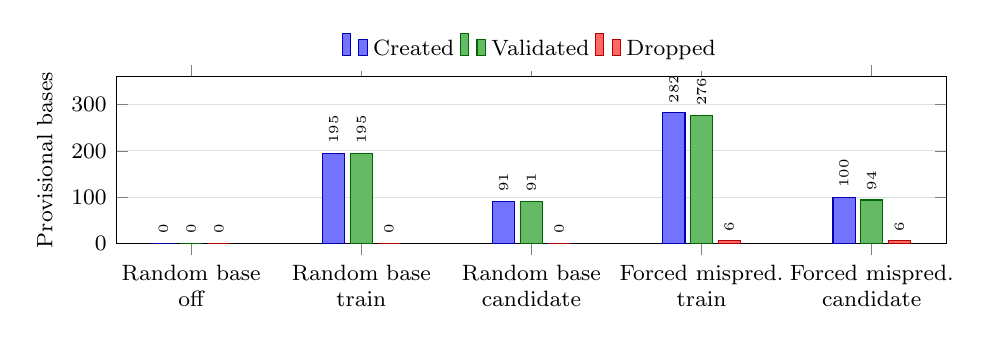
\begin{tikzpicture}
    \begin{axis}[provbar, bar width=8pt, ymax=360,
                 ylabel={Provisional bases}]
        \addplot[fill=blue!55, draw=blue!70!black] coordinates
            {(RBoff,0) (RBtrain,195) (RBcand,91) (FMtrain,282) (FMcand,100)};
        \addplot[fill=green!55!black!60, draw=green!40!black] coordinates
            {(RBoff,0) (RBtrain,195) (RBcand,91) (FMtrain,276) (FMcand,94)};
        \addplot[fill=red!60, draw=red!70!black] coordinates
            {(RBoff,0) (RBtrain,0) (RBcand,0) (FMtrain,6) (FMcand,6)};
        \legend{Created, Validated, Dropped}
    \end{axis}
    \end{tikzpicture}

    \vspace{0.2em}

    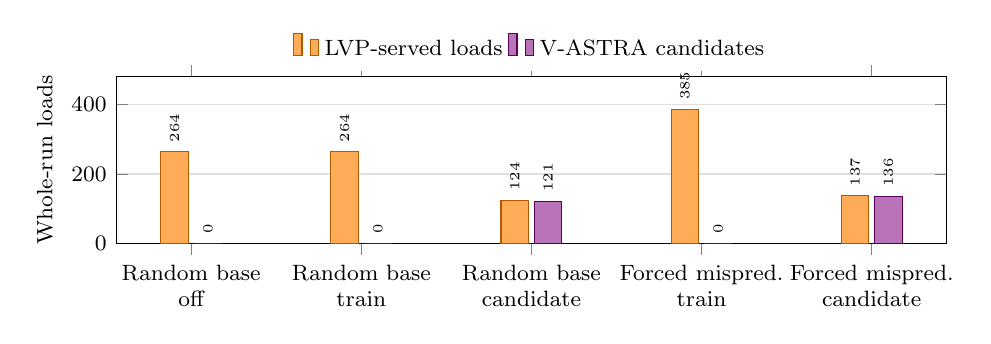
\begin{tikzpicture}
    \begin{axis}[provbar, bar width=10pt, ymax=480,
                 ylabel={Whole-run loads}]
        \addplot[fill=orange!65, draw=orange!70!black] coordinates
            {(RBoff,264) (RBtrain,264) (RBcand,124) (FMtrain,385) (FMcand,137)};
        \addplot[fill=violet!55, draw=violet!70!black] coordinates
            {(RBoff,0) (RBtrain,0) (RBcand,121) (FMtrain,0) (FMcand,136)};
        \legend{LVP-served loads, V-ASTRA candidates}
    \end{axis}
    \end{tikzpicture}

    \caption{Provisional-base results. Top: provisional bases
    created, validated, and dropped. Bottom: LVP-served loads
    and the V-ASTRA candidates formed from them over the whole run
    (candidacy does not apply in \texttt{off} mode).}
    \label{tab:meta-provisional-results}
\end{figure}

No provisional producer published a forwarding record in any mode. In
the random-base \texttt{candidate} run, every candidate had ASTRA's
predicted base equal to the LVP operand.

These results show that \texttt{train} mode prevents provisional
LVP-fed loads from becoming V-ASTRA candidates, while
\texttt{candidate} mode permits candidate formation using the
provisional operand. The forced-misprediction run in candidate mode
directly demonstrates that
eight consumers can bypass before operand validation and are
subsequently discarded after the wrong-used LVP prediction is
detected. It does not demonstrate that the LVP operand was correct at
the time it was used. Correctness is enforced through later validation
and recovery, not by requiring validation before candidate use.

\subsubsection{Forced Misprediction and Recovery Ordering}
\label{subsubsec:meta-forced-misprediction-recovery}

Under META, an incorrect LVP prediction triggers recovery only if a
consumer has actually used it. The producer is marked
\texttt{lvpUsedBySpec} only after the consumer's request is accepted
into the LSQ. When the producer responds, its prediction is compared
with the actual value and the predictor is trained. If the prediction
was incorrect and \texttt{lvpUsedBySpec} is set, execution redirects
to the producer's next PC, discarding younger instructions.

The implementation also checks that a consumer's architectural source
matches the value it used and that an incorrectly validated producer
with live LVP users triggers recovery. Multiple live users are tracked,
with a drain-time check ensuring none remain.

Four directed cases distinguish incorrect predictions from incorrect
predictions that were used:
\begin{itemize}
    \item \textbf{Wrong value used:} Three recoveries occurred, matching
    the LVP-only control.

    \item \textbf{Wrong value not used:} Three incorrect predictions
    caused no recovery, unlike the three recoveries in the LVP-only
    control.

    \item \textbf{V-ASTRA consumers:} Three incorrect LVP predictions
    caused no LVP recovery. Four consumers used V-ASTRA values instead.

    \item \textbf{Forced misprediction:} Nine wrong-used predictions
    each caused a redirect, and all affected consumers were discarded
    before commit.
\end{itemize}

The forced-misprediction case reports nine wrong-used predictions and
nine redirects in whole-run traces, but six recovery events in statistics. These counts have different measurement scopes. In
candidate mode, eight consumers were bypassed before operand
validation. For each, the trace confirmed the non-decreasing event
order:
\[
\text{bypass} \rightarrow \text{validation} \rightarrow
\text{redirect} \rightarrow \text{discard}.
\]
None committed. The same nine wrong-used predictions were recovered
in \texttt{off}, \texttt{train}, and \texttt{candidate} modes.

The tests do not demonstrate one producer with several direct LVP
consumers all being squashed together. Multiple-user tracking is
implemented, but this specific pattern was not observed in the
forced-misprediction workload.

\subsubsection{Alignment and Provisional-State Retry Regression}
\label{subsubsec:meta-alignment-retry}

The pre-fix regression reproduced a cleanup defect when an LVP-fed
load captured a provisional ASTRA base but faulted on misalignment
before LSQ insertion. On re-execution, the stale provisional state
remained and caused a commit-time assertion failure. The fix clears
leftover provisional state at the start of each new
\texttt{astraCaptureBase} attempt.

The post-fix regression passed all 92 checks across four
configurations: no prediction, and META with
\texttt{metaAstraLvpLoads} set to \texttt{off}, \texttt{train}, and
\texttt{candidate}. It recorded 60 provisional bases created and
60 dropped, matching the 60 early alignment faults. Each faulting
attempt was followed by one head-of-pipeline re-execution, with no
architectural faults or training on a misaligned base. Output and
committed values matched the no-predictor control across 2,611
instructions.

The test exercises no V-ASTRA bypass: the alignment faults occur
before LSQ insertion, resulting in zero accepted consumers and zero
bypasses of the faulting load. Repeated retries, post-LSQ faults, and
translation faults on provisional loads remain untested. The result
therefore validates the specific early-alignment-fault cleanup path,
not provisional-state recovery in general.
